\documentclass{beamer}

% \usepackage{beamerthemesplit} // Activate for custom appearance
\usepackage{graphicx}
\DeclareGraphicsExtensions{.pdf,.png}

\usetheme{Berkeley}
\usecolortheme{seagull}
\usefonttheme{structuresmallcapsserif}

\newcommand{\tab}{\hspace*{2em}}

\title[Tools]{Internal Tools}
\author{James Condron}
\date{\today}

\begin{document}

\frame{\titlepage}

\frame{\tableofcontents}
\section{Definitions}
\frame{
  \frametitle{What is http?}
  \begin{itemize}
  \item The {\tt HyperText Transfer Protocol}
  \item Uses a *request/response* model
  \item Consists of a Verb, a Path, a Version and then headers
  \item Defined at http://www.w3.org/Protocols/rfc2616/rfc2616.html
  \end{itemize}
}

\frame{
  \frametitle{HTTP/1.0 and HTTP/1.1}
  \begin{itemize}
  \item {\tt HTTP/1.0} is very basic, handled simple pages and forms
  \item {\tt HTTP/1.1} is richer and what we use today
  \item Requests made with {\tt HTTP/1.1} must include extra information
 \end{itemize}
}


\frame{
  \frametitle{TEH INTERNETZ}
  HTTP is used for two (main) things
  \begin{itemize}
  \item Passing html to a browser for human consumption
  \item Passing data via an API for computer consumption
  \end{itemize}
}

\frame{
  \frametitle{API?}
 \begin{itemize}
  \item Application Programmer's Interface
  \item Data in a format a computer can understand
  \end{itemize}
}

\section{Requests}
\frame{
  \frametitle{Everything Is Requests}
  \begin{itemize}
  \item I will be using a very simple API of my own to demonstrate HTTP
  \item And will call the API with 'curl'
  \end{itemize}
}

\subsection{Verbs}
\frame{
  \frametitle{Basics}
  \begin{itemize}
  \item The simplest three verbs to understand are *GET*, *HEAD* and *POST*
  \item These were defined in HTTP/1.0
  \item Every time you visit a website your browser performs a 'GET'
  \end{itemize}
}

\frame{
  \frametitle{Basics (Cont.)}
  \begin{figure}[h]
    \centering
    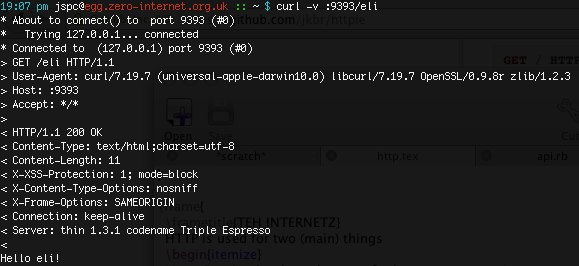
\includegraphics[height=2.5in]{img/get.png}
    \caption{GET request on '/eli'}
    \label{fig:get}
   \end{figure}
}

\frame{
  \frametitle{GET}
  \begin{itemize}
  \item First defined under {\tt HTTP/1.0}
  \item Must include the URI to query and the Host on which to do so
  \end{itemize}
}

\frame{
  \frametitle{GET (Cont.)}
  \begin{figure}[h]
    \centering
    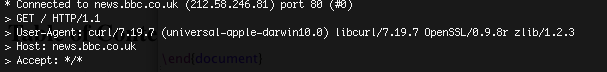
\includegraphics[height=2.5in]{img/get_req.png}
    \caption{GET request on '/'}
    \label{fig:get request full}
   \end{figure}
}

\frame{
  \frametitle{POST}
  \begin{itemize}
  \item Also first defined under {\tt HTTP/1.0}
  \item We use this to send form data
  \item It takes data in {\tt key=value} form
  \item Each pair is seperated with {\tt &}
 \end{itemize}
}

\frame{
  \frametitle{POST (Cont.)}
  \begin{figure}[h]
    \centering
    
\includegraphics[height=2.5in]{img/post_req.png}
    \caption{POST request to '/person/me'}
    \label{fig:post request full}
   \end{figure}
}

\section{Responses}
\frame{
  \frametitle{Basics}
  \begin{itemize}
  \item Every request returns a response
  \item Usually this has some kind of data; a website or status
  \item They always have a response code
  \end{itemize}
}

\frame{
  \frametitle{Basics (Cont.)}
  \begin{figure}[h]
    \centering
    
\includegraphics[height=2.5in]{img/500_cat.jpg}
    \caption{POST request to '/person/me'}
    \label{fig:post request full}
   \end{figure}
}

\frame{
  \frametitle{1xx Response}
  \begin{itemize}
  \item Purely informational/ 'Request Received'
  \item Didn't exist in {\tt HTTP/1.0}
  \item Rarely need to use 1xx codes
  \end{itemize}
}

\frame{
  \frametitle{2xx Response}
  \begin{itemize}
  \item SUCCESS!!!!!!11111!111!!w33
  \item Generally use 200
  \item These statuses tell the requester that whatever they were trying to do worked
  \end{itemize}
}

\frame{
  \frametitle{3xx Response}
  \begin{itemize}
  \item Redirection
  \item These tell the requester that whatever it was they're looking for lives elsewhere
  \item These are important to catch: usually we want to follow redirects to get to where we want to be
  \end{itemize}
}

\frame{
  \frametitle{4xx Response}
  \begin{itemize}
  \item Client Side Error
  \item These mean the requester made a boo-boo
  \item Take {\tt 404} errors- the resource you want doesn't exist
  \item Or {\tt 403} - you're not allowed to see it
  \item {\tt 418} means ``I'm a teapot''
  \end{itemize}
}

\frame{
  \frametitle{5xx Response}
  \begin{itemize}
  \item These are *server* errors
  \item {\tt 503} errors, for example, means 'Servcie Unavailable'
 \end{itemize}
}


\end{document}
